\documentclass{VUMIFPSkursinis}
\usepackage{algorithmicx}
\usepackage{algorithm}
\usepackage{algpseudocode}
\usepackage{amsfonts}
\usepackage{amsmath}
\usepackage{bm}
\usepackage{caption}
\usepackage{color}
\usepackage{float}
\usepackage{graphicx}
\usepackage{listings}
\usepackage{subfig}
\usepackage{wrapfig}


\usepackage{enumitem}
%PAKEISTA, tarpai tarp sąrašo elementų
\setitemize{noitemsep,topsep=0pt,parsep=0pt,partopsep=0pt}
\setenumerate{noitemsep,topsep=0pt,parsep=0pt,partopsep=0pt}

% Titulinio aprašas
\university{Vilniaus universitetas}
\faculty{Matematikos ir informatikos fakultetas}
\department{}
\papertype{Informacinių sistemų pirmas laboratorinis darbas}
\title{Žaidimų pristatymų „Another One" įmonės informacinė sistema ir jos analizė}
\titleineng{}
\status{Programų sistemų 4 kurso studentai}
\author{Nedas Valentinovičius, Linas Valiukonis}
\supervisor{Audronė Lupeikienė, M. Darbuot., Dr.}
\date{Vilnius – \the\year}

% Nustatymai
%\setmainfont{Palemonas}
% \bibliography{bibliografija}

\newcommand{\tabitem}{~~\llap{\textbullet}~~}
\newcommand{\tabitemd}{~~\llap{\textopenbullet}~~}

\renewcommand{\labelenumii}{\theenumii}
\renewcommand{\theenumii}{\theenumi.\arabic{enumii}.}

\begin{document}
	
\maketitle
\cleardoublepage\pagenumbering{arabic}
\setcounter{page}{2}

\sectionnonum{Anotacija}
Komandos nariai ir jų kontaktiniai duomenys:
\begin{itemize}
	\item Linas Valiukonis, paštas: linas.valiukonis@mif.stud.vu.lt
	\item Nedas Valentinoviičus, paštas: nedas.valentinovičius@mif.stud.vu.lt
\end{itemize}
Grupės narių indėliai:
\begin {itemize}
	\item Linas Valiukonis - 50\%
	\item Nedas Valentinovičius - 50\%
\end{itemize}

\tableofcontents

\sectionnonum{Įvadas}
Šiame dokumente yra pateikiamas žaidimų pristatymo „Another One" įmonės informacinės sistemos (toliau IS) aprašas. Egzistuojančio verslo pavyzdys galėtų būti bet kokia internetinė parduotuvė vykdanti užsakymus. Mūsų paslaugomos skelbiamos mūsų internetinėje svetainėje, taip pat reklamos kituose tinklalapiuose. Mes pristatom klientams jų prekes, sudarom sutartis su kitomis įmonėmis, kad jos galėtų naudotis mūsų sukurtu įrankiu (internetiniu puslapiu).

\section{Panaudotų dokumentų sąrašas}

%\begin{figure}[H]
%    \centering
%    \includegraphics[scale=0.8]{img/Procesudiagrama}
%    \caption{Kūrimo procesų diagrama}
%    \label{img:mlp}
%\end{figure}


\newpage
\section{Kompiuterizuojamo objekto anazilė}

\newpage
\subsection{Kompiuterizuojamo verslo objekto apibūdinimas}
Žaidimų pristatymo įmonės „Another One" verslo sistema pristato klientų įgytas prekias jiems fizižkai ar virtualiai. Paslaugos yra reklamuojamos internetinėje įmonės svetainėje. Sudaromos sutartys su kitomis įmonėmis, kurios nori pasinaudoti mūsų sistema ir išplatinti jų produktus.
\begin{center}
\begin{table}[ht]
\centering
	\caption{Kokybės užtikrinimo procesas}
	\begin{tabular}{| p{0.1\linewidth} | p{0.9\linewidth }|} 
	\hline
	Kodėl  & Verslo strategija - auginti klientų lojalumą, trumpinti pristatymo laikus, vykdyti apmokymus darbuotojams.\\ 
		&\\
		& Verslo vizija - įmonė turėdama lojalių klientų, augina paslaugų ir parduodamų prekių kiekį, išlaiko klientų bazė rinkoje. \\
		&\\
		& SWOT analizė: \\
		&\hspace{4mm}\tabitem Stiprybės: \\ 
		&\hspace{8mm}\tabitemd didelis prekių pasirinkimas, \\
		&\hspace{8mm}\tabitemd klientas gali iškart gauti prekę. \\
		&\hspace{4mm}\tabitem Silpnybės: \\
		&\hspace{8mm}\tabitemd mažas darbuotojų skaičius, aukštas klientų skaičius (švenčių laikotarpiu), \\
		&\hspace{8mm}\tabitemd planavimo sunkumai su atvykstančiomis prekėmis, nežinomas prekių kiekis sandelyje (nėra galimybės greitai patikrinti). \\
		&\hspace{4mm}\tabitem Galimybės: \\
		&\hspace{8mm}\tabitemd kompiuterizuota sistema padėtų valdyti atvykstančias prekes bei suteiktu klientams galimybę užsisakyti internetu, \\
		&\hspace{8mm}\tabitemd pasasmdžius daugiau darbuotojų būtų aptarnaujama daugiau klientų vienu metu, padidėtų produktyvumas ir pelnas. \\
		&\hspace{4mm}\tabitem Rizikos: \\
		&\hspace{8mm}\tabitemd augant darbuotojų skaičiui bus sunkiau kokybiškai juos visus apmokyti, \\
		&\hspace{8mm}\tabitemd verslas bankrutuos jei bus pandemija. \\ \hline
	Kaip 	&  Verslo transakcijos: produkto užsakymo priėmimas, apmokėjimas už produktą, produktų pirkimas, produktų atvežimas. \\ \hline
	Kas 	& Verlslo objektai: produktai (žaidimai, žaidimų konsolės, įranga ir kt.), klientai, darbuotojai, pinigai, banko kortelės, transporto priemonės. \\ \hline
	Kam 	& Suinteresuotieji asmenys: klientai, darbuotojai, užsakovai (iš kurių gauname produktus). \\ \hline
	Kur 	& Prieigos taškai: \\
		&\hspace{4mm}\tabitem įmonės parduotuvė - klientai perka gyvai.\\ 
		&\hspace{4mm}\tabitem įmonės biuras - įmonės direktorius arba administratorius registruoja atvykstančius produktus į lokalius failus (kiek kokių produktų atvyko siunta). \\ \hline
	Kada 	& Laiko apribojimai: klientai perka jau esamas prekes. Užsakymai iš tiekėjų yra įrašomi į lokalius failus su numatyta atvežimo data ir laiku bei užsakymo pradžios laiku\\ \hline				\end{tabular}
\end{table}	
\end{center}
\newpage
\subsection{IS konteksto diagrama. IS išoriniai informacijos srautai}
\begin{figure}[H]
    \centering
    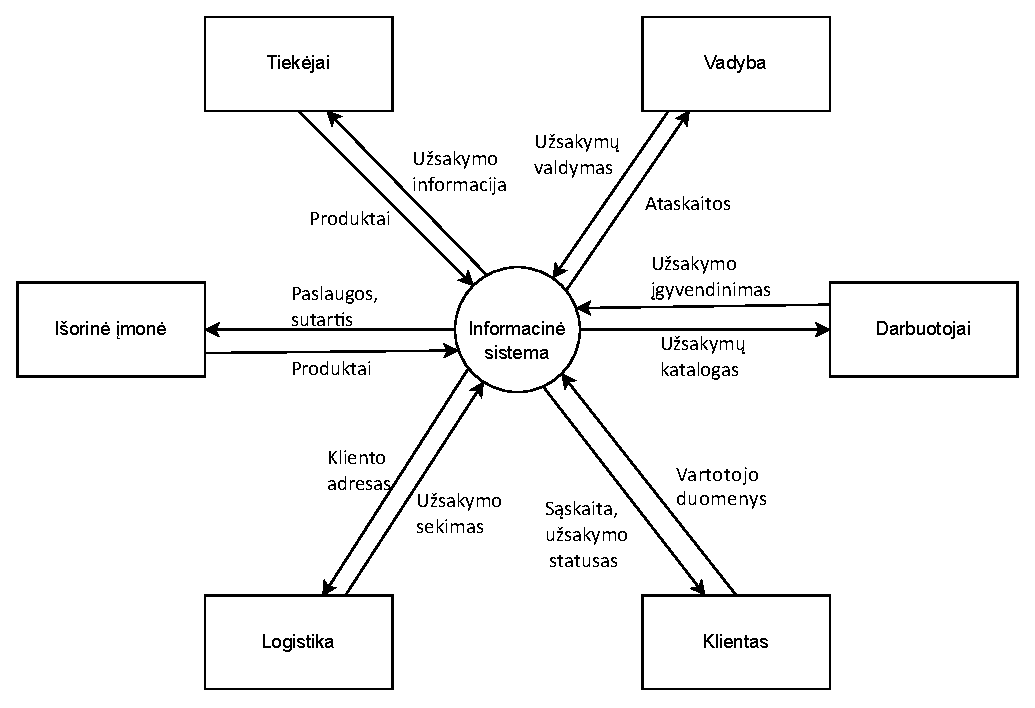
\includegraphics[scale=1]{img/KontekstoDiagrama2}
    \caption{Konteksto diagrama}
    \label{img:mlp}
\end{figure}
Informacinės sistemos išorinių informacijos/duomenų srautų aprašai:
\begin{enumerate}
	\item Šaltinis - Klientas
	\begin{enumerate}
		\item Identifikatorius: ORD
		\item Duomenų aprašymas: iš kliento tapatybė patvirtinantis dokumentas, užsakymo informacija. \\ Mūsų įmonė perduoda sąskaita bei užsakymo statusą.
		\item Periodiškumas: kai klientas padaro užsakymą.
		\item Duomenų formatas: skaitmeniniai dokumentai. 
		\item Duomenų perdavimo būdas: elektroninis paštas.
	\end{enumerate}
	\item Šaltinis - Logistika
	\begin{enumerate}
		\item Identifikatorius: LGX
		\item Duomenų aprašymas: už logistika atsakinga įmonė pateikia užsakymo sekimo informacija. \\ Mūsų įmonė perduoda kliento adresą bei siuntos informaciją.
 		\item Duomenų srauto apimtis (kiekis per dieną): vieną kartą.
		\item Duomenų formatas: skaitmeniniai dokumentai, popieriniai dokumentai.
		\item Duomenų perdavimo būdas: per internetą arba tiesioginiu būdu.
	\end{enumerate}
	\item Šaltinis - Išorinė įmonė
	\begin{enumerate}
		\item Identifikatorius: DL
		\item Duomenų aprašymas: išorinė įmonė pateikia mums produktų informacija, kaip nori naudotis mūsų paslaugomis. \\ Mūsų įmonė perduoda paslaugų informacija.
		\item Periodiškumas: kai abi pusės susitaria ir pasirašo sutartį.
		\item Duomenų formatas: popieriniai dokumentai
		\item Duomenų perdavimo būdas: tiesioginis
	\end{enumerate}
	\item Šaltinis - Tiekėjai
	\begin{enumerate}
		\item Identifikatorius: SUPP
		\item Duomenų aprašymas: pateikia produktų informacija ir sąskaitą. \\ Mūsų įmonė pateikia užsakymo informacija.
		\item Periodiškumas: pagal sutartį numatytą periodiškumą arba kai sudaroma sutartis.
		\item Duomenų formatas: popieriniai dokumentai.
		\item Duomenų perdavimo būdas: tiesioginis
	\end{enumerate}
	\item Šaltinis - Vadyba
	\begin{enumerate}
		\item Identifikatorius: MNG
		\item Duomenų aprašymas: perduoda nurodymus, kuriuos užsakymus vykdyti, įrašus kada kokios siuntos atvyks. \\ Mūsų įmonė perduoda siuntų ataskaitas.
 		\item Duomenų srauto apimtis (kiekis per dieną): iki 3~5 kartų
		\item Duomenų formatas: skaitmeniniai dokumentai.
		\item Duomenų perdavimo būdas: internetinės operacijos.
	\end{enumerate}
	\item Šaltinis - Darbuotojai
	\begin{enumerate}
		\item Identifikatorius: WKR
		\item Duomenų aprašymas: atnaujinta informacija apie užsakymą, laikas ir pastabos apie užsakymą. \\ Mūsų įmonė perduoda užsakymų katalogą bei nurodymus iš vadybos.
 		\item Duomenų srauto apimtis (kiekis per valandą): apie 12
		\item Duomenų formatas: skaitmeniniai dokumentai arba popieriniai dokumentai.
		\item Duomenų perdavimo būdas: internetinės užklausos, tiesioginis.
	\end{enumerate}
\end{enumerate}

\newpage
\subsection{IS galimybių medis}
Sistema turi:
\begin{enumerate}
	\item Pateikti produktų sąrašą.
	\item Priimti ir išsaugoti klientų užsakymus.
	\item Pateikti klientui užsakymo anksčiausia atvykimo laiką.
	\item Apskaičiuoti užsakymo kainą.
	\item Užregistruoti užregistruoti, kai klientas sumoką už užsakymą.
	\item Pateikti darbuotojų sąrašą.
	\item Leisti redaguoti darbuotojų sąrašą.
	\item Pateikti užsakymų katalogą.
	\item Leisti redaguoti užsakymų katalogą.
	\item Pateikti produktų katalogą.
	\item Leisti redaguoti produktų katalogą.
	\item Leisti skelbti akcijas ir naujienas.
\end{enumerate}
\begin{figure}[H]
    \centering
    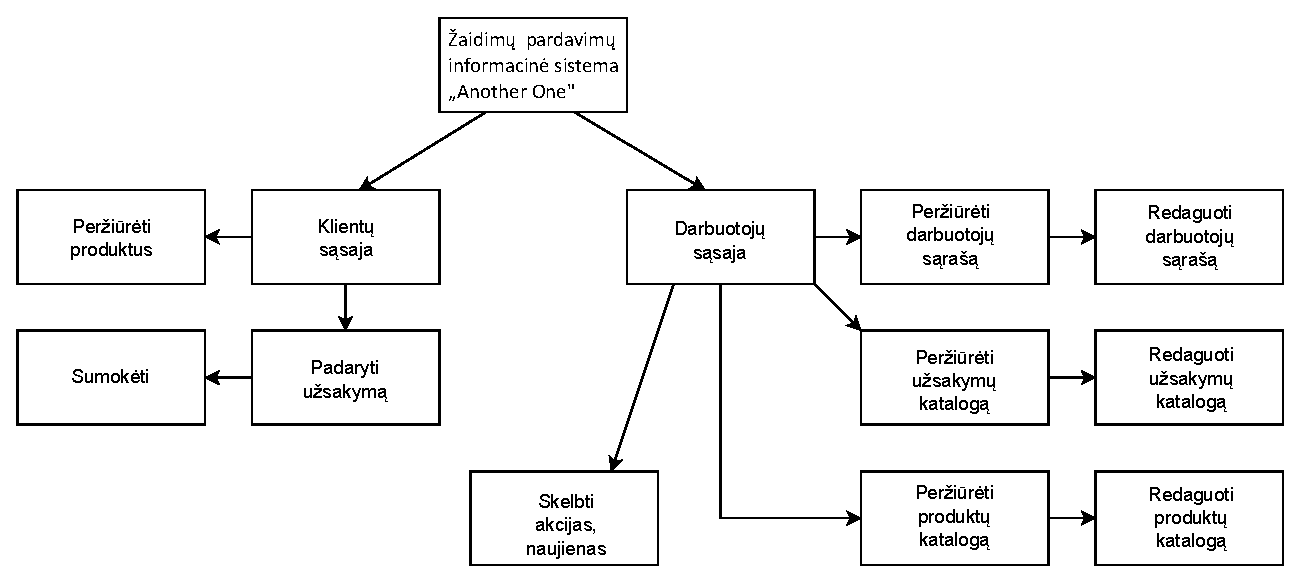
\includegraphics[scale=0.8]{img/GalimybiuMedis}
    \caption{Galimybių medis}
    \label{img:mlp}
\end{figure}

\newpage
\subsection{IS užduotys}
Šiame skyriuje bus išnagrinėtos verslo užduotys iš \ref{img:UC} diagramos ir iš jų bus sudaromos IS užduotys.
\begin{figure}[H]
    \centering
    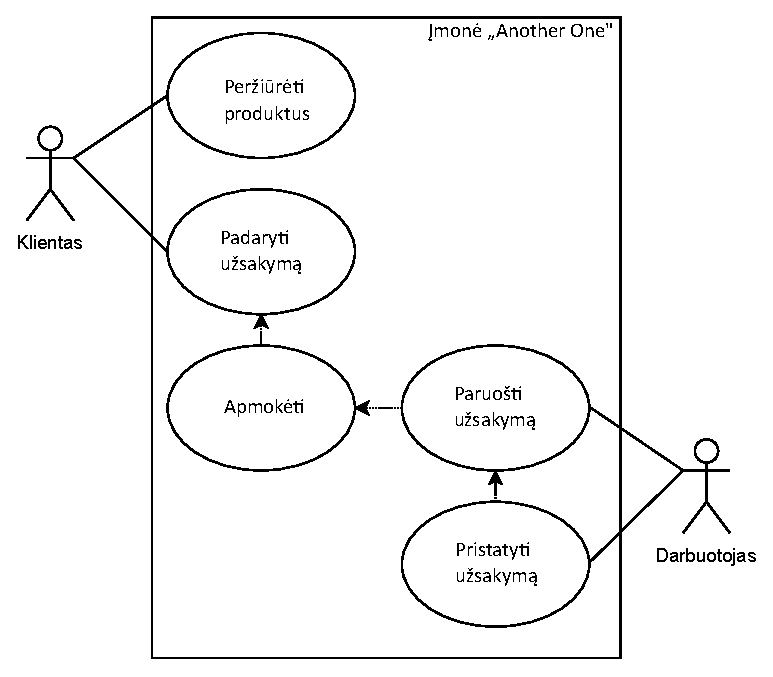
\includegraphics[scale=1]{img/UseCase}
    \caption{Verslo užduoių diagrama}
    \label{img:UC}
\end{figure}

\begin{enumerate}
	\item Peržiūrėti produktus
	\begin{enumerate}
		\item Procesai: atvykti į fizinę parduotuvę/apsilankyti internetiniame puslapyje, peržiūrėti produktus ir jų informacija.
		\item Produkto naudojimo atvejis: produktų katalogo pateikimas.
	\end{enumerate}
	\item Padaryti užsakymą
	\begin{enumerate}
		\item Procesai: atvykti į fizinę parduotuvę/apsilankyti internetinėje svetainėje, peržiūrėti produktus, išsirinkti norimus produktus, pateikti reikalinga informaciją reikalingą užsakymo sukūrimui, apmokėti, užregistruoti užsakymą į užsakymų katalogą.
		\item Produkto naudojimo atvejis: produktų katalogo pateikimas, užsakymo sukūrimas, užsakymo apmokėjimas, užsakymo įrašymas į užsakymų katalogą.
	\end{enumerate}
	\item Apmokėti
	\begin{enumerate}
		\item Procesai: apmokėti už produktą fizinėje parduotuvėje banko kortele/grynais arba internetu per elektroninę bankininkystę.
		\item Produkto naudojimo atvejis: apmokėjimo atlikimas.
	\end{enumerate}
	\item Paruošti užsakymą
	\begin{enumerate}
		\item Procesai: peržiūrėti užsakymų katalogą, supakuoti užsakymą pristatymui, pakeisti užsakymo statusą užsakymų kataloge.
		\item Produkto naudojimo atvejis: Užsakymo katalogo pateikimas, užsakymo katalogo pakeitimas.
	\end{enumerate}
	\item Pristatyti užsakymą
	\begin{enumerate}
		\item Procesai: peržiūrėti užsakymų katalogą, paimti užsakymą, pristatyti užsakymą, pakeisti užsakymo statusą užsakymų kataloge.
		\item Produkto naudojimo atvejis: Užsakymo katalogo pateikimas, užsakymo katologo pakeitimas, pranešimo, apie siuntos pristatymą, išsiuntimas.
	\end{enumerate}
\end{enumerate}

\begin{figure}[H]
    \centering
    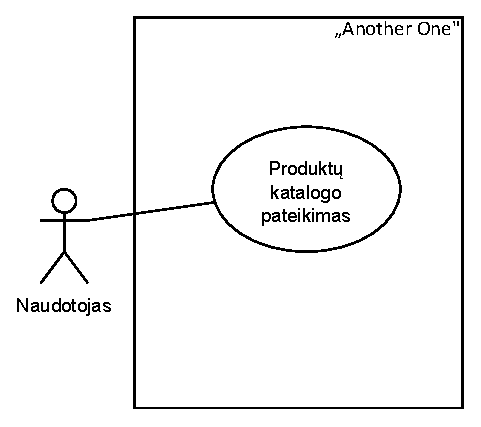
\includegraphics[scale=1]{img/ProductUseCase1}
\end{figure}
\begin{figure}[H]
    \centering
    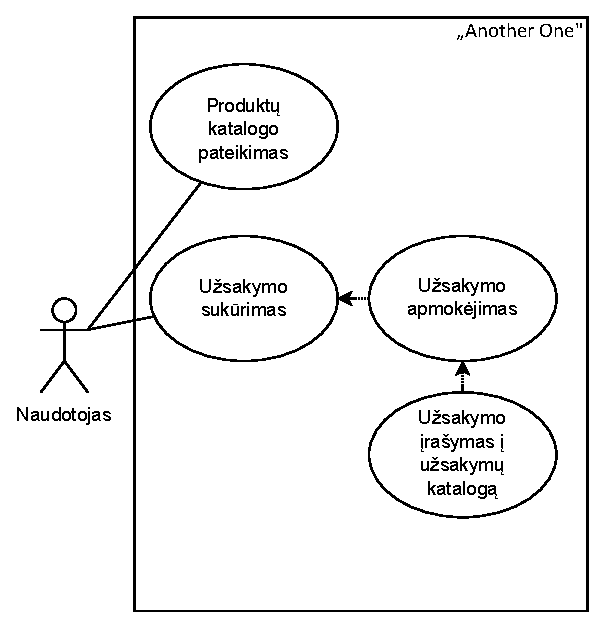
\includegraphics[scale=1]{img/ProductUseCase2}
\end{figure}
\begin{figure}[H]
    \centering
    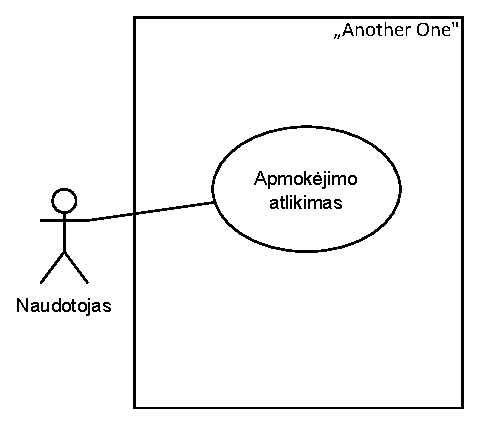
\includegraphics[scale=1]{img/ProductUseCase3}
\end{figure}
\begin{figure}[H]
    \centering
    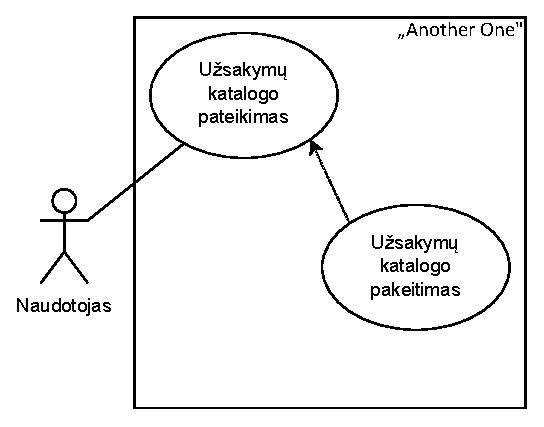
\includegraphics[scale=1]{img/ProductUseCase4}
\end{figure}
\begin{figure}[H]
    \centering
    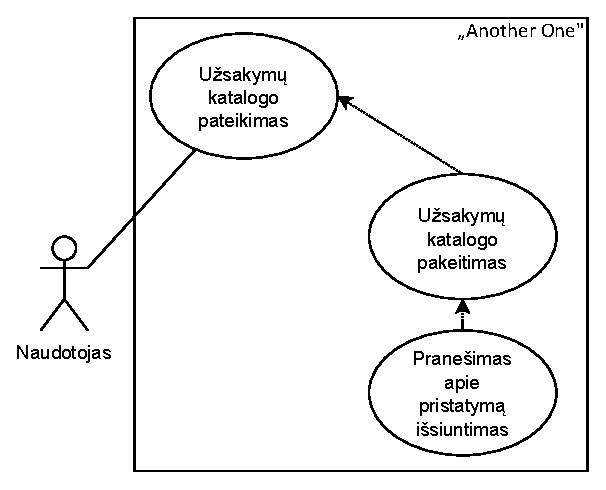
\includegraphics[scale=1]{img/ProductUseCase5}
\end{figure}

\newpage
\subsection{IS saugoma informacija (saugyklos)}
Esminių esybių (vartotojai, darbuotojai, užsakymai ir produktai) duomenys bus saugomi SQL duomenų bazėje. Ryšiai tarp esybių matomi \ref{img:RS} diagramoje. „User" lentelėje saugomi duomenys apie vartotoją (vardas, kontaktiniai duomenys). „Order" lentelėje saugmi duomenys apie užsakymus (kas užsakė, kas paruošė užsakymą, kokie produktai įeina į užsakymą ir kt.). „Worker" lentelėje saugomi duomenys apie darbuotojus (darbuotojo vardas, kontaktiniai duomenys, darbuotojo ID). „Product" lentelėje saugoma informacija apie produktus. \\
Duomenis galima atvaizduoti kompiuterio ekrane.
\begin{figure}[H]
    \centering
    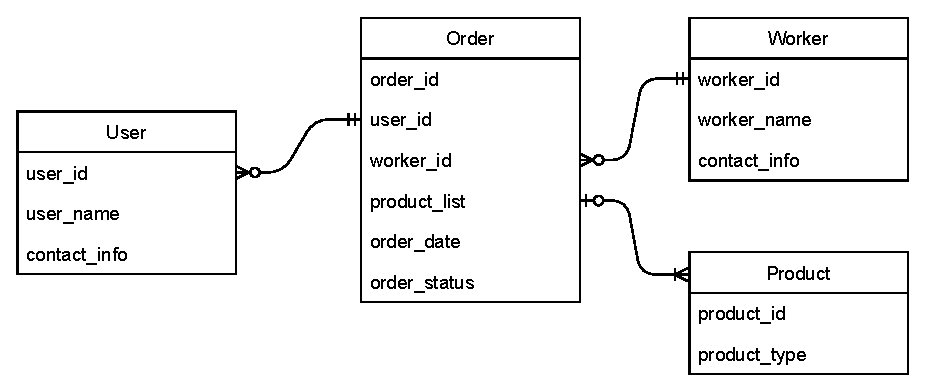
\includegraphics[scale=1]{img/RealiacineSchema}
    \caption{Esminių esybių reliacinė schema}
    \label{img:RS}
\end{figure}

\newpage
\subsection{Informacijos apdorojimo procesai}

\newpage
\subsection{IS vartotojai ir jų darbo vietos}

\newpage
\subsection{IS inžinieriaus požiūris. Užpildoma antra 1 lentelės eilutė}

\newpage
\subsection{Sudaromas IS posistemių sąrašas ir nurodomi jų tipai}

\newpage
\subsection{IS registrų sistema}

\newpage
\section{Pastabos apie dokumentą DĖL VALSTYBĖS INFORMACINIŲ SISTEMŲ GYVAVIMO CIKLO VALDYMO METODIKOS PATVIRTINIMO}

\newpage

\section{Išvados}

\newpage
\sectionnonum{Terminų žodynėlis}
\begin{itemize}
	\item{Trikdžiai -- veikla ar procesus stabdantys veiksniai}
\end{itemize}

\section{Priedai}

\newpage
\section{Pavyzdiniai latexo dalykai, nes dažnai pamirštu}
Citavimo pavyzdžiai: cituojamas vienas šaltinis \cite{PvzStraipsnLt}; cituojami
keli šaltiniai \cite{PvzStraipsnEn, PvzKonfLt, PvzKonfEn, PvzKnygLt, PvzKnygEn,
PvzElPubLt, PvzElPubEn, PvzMagistrLt, PvzPhdEn}.

\begin{enumerate}
	\item Pirmas elementas
	\item Antras elementas
\end{enumerate}

\begin{figure}[H]
    \centering
    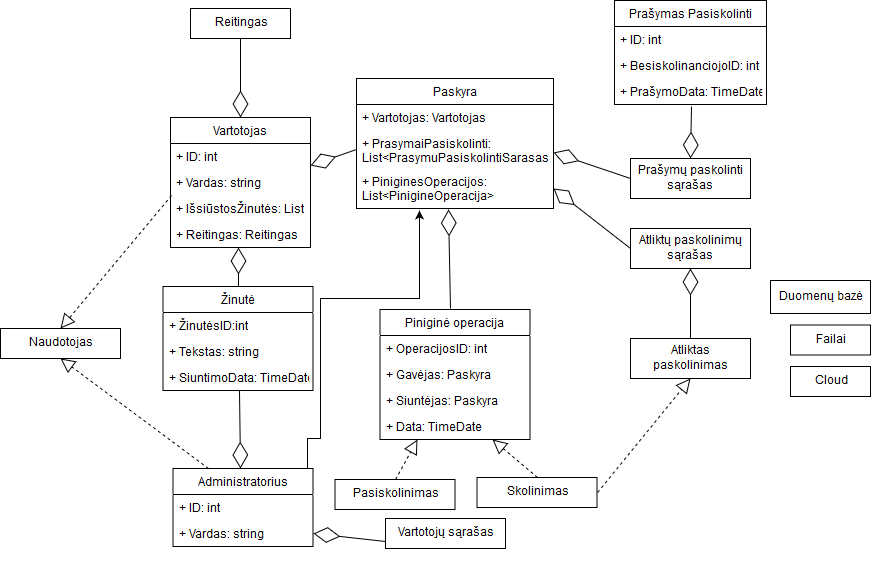
\includegraphics[scale=0.5]{img/DomainModel}
    \caption{Paveikslėlio pavyzdys}
    \label{img:mlp}
\end{figure}

% tablesgenerator.com - converts calculators (e.g. excel) tables to LaTeX
\begin{table}[H]\footnotesize
  \centering
  \caption{Lentelės pavyzdys}
  {\begin{tabular}{|l|c|c|} \hline
    Algoritmas & $\bar{x}$ & $\sigma^{2}$ \\
    \hline
    Algoritmas A  & 1.6335    & 0.5584       \\
    Algoritmas B  & 1.7395    & 0.5647       \\
    \hline
  \end{tabular}}
  \label{tab:table example}
\end{table}

\end{document}